\documentclass[11pt,letterpaper]{article}
\usepackage[lmargin=1in,rmargin=1in,tmargin=1in,bmargin=1in]{geometry}
\usepackage{../style/homework}
\usepackage{../style/commands}
\setbool{quotetype}{true} % True: Side; False: Under
\setbool{hideans}{false} % Student: True; Instructor: False

% -------------------
% Content
% -------------------
\begin{document}

\homework{12: Due 04/14}{I was very slow in maths, geometry I actually enjoyed.}{Liam Neeson}

% Problem 1
\problem{10} Find the volume and surface area of the right circular cone shown below. [Note: Assume the line segment of length 8 below passes through the center of the circle.]
	\[
	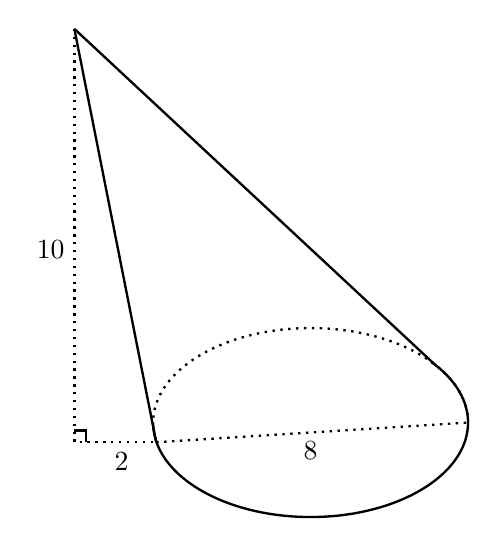
\begin{tikzpicture}
	\draw[line width=0.03cm] (-1.96,-0.25) -- (-3,5);
	\draw[line width=0.03cm] (1.58,0.735) -- (-3,5);    
	                                                           
	\draw[line width=0.03cm,dotted] (-3,5) -- (-3,-0.25) -- (-1.96,-0.25);
	\draw[line width=0.03cm] (-3,-0.1) -- (-2.85,-0.1) -- (-2.85,-0.25);
	\node at (-3.3,2.2) {$10$};
	
	\draw[line width=0.03cm,dotted] (-1.96,-0.25) -- (2,0);
	\node at (0,-0.35) {$8$};
	
	\node at (-2.4,-0.5) {$2$};
	
	\draw[line width=0.03cm,dotted] (2, 0) arc [start angle=0, end angle=180, x radius= 2, y radius= 1.2];
	\draw[line width=0.03cm] (-2, 0) arc [start angle=180, end angle=400, x radius= 2, y radius= 1.2];	
	\end{tikzpicture}
	\] \pspace

\sol The volume of a circular cone is $V= \frac{1}{3} \cdot \pi r^2 \cdot h$. But then we have\dots
	\[
	V= \frac{1}{3} \cdot \pi r^2 \cdot h= \frac{1}{3} \cdot \pi \cdot \left( \frac{8}{2} \right)^2 \cdot 10 \approx 167.552
	\]
The surface area of a circular cone is $\pi r^2 + \pi r s$. We know that $s= \sqrt{10^2 + 10^2}= \sqrt{200}$. But then we have\dots
	\[
	\text{SA}= \pi r^2 + \pi r s= \pi \cdot 4^2 + \pi \cdot 4 \cdot \sqrt{200} \approx 227.981
	\]



\newpage



% Problem 2
\problem{10} Find the volume and surface area of the right circular cylinder with diameter 3 and height 10 shown below.
	\[
	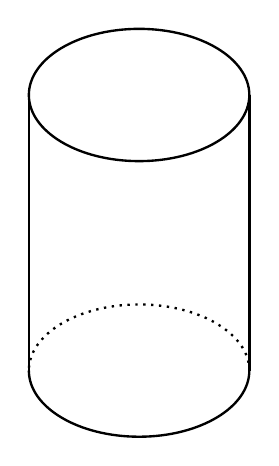
\begin{tikzpicture}[scale=0.7]
	\draw[line width=0.03cm] (0,5) ellipse (2 and 1.2);
	\draw[line width=0.03cm] (-2,5) -- (-2,0);
	\draw[line width=0.03cm] (2,5) -- (2,0);
	\draw[line width=0.03cm,dotted] (2, 0) arc [start angle=0, end angle=180, x radius= 2, y radius= 1.2];
	\draw[line width=0.03cm] (-2, 0) arc [start angle=180, end angle=360, x radius= 2, y radius= 1.2];
	\end{tikzpicture}
	\] \pspace

\sol The volume of a circular cylinder is $\pi r^2 h$. The cylinder has diameter 3, i.e. radius 1.5. But then we have\dots
	\[
	V= \pi r^2h= \pi \cdot 1.5^2 \cdot 10 \approx 70.6858
	\]
The surface area of a circular cylinder is $2\pi r^2 + 2\pi r h$. But then we have\dots
	\[
	\text{SA}= 2\pi r^2 + 2\pi r h= 2 \pi \cdot 1.5^2 + 2 \pi \cdot 1.5 \cdot 10 \approx 14.1372 + 94.2478 \approx 108.385
	\]



\newpage



% Problem 3
\problem{10} Find the volume and surface area of the cube shown below. Also, find the length of the `diagonal' of the cube, i.e. the length from one corner to another. 
 	\[
	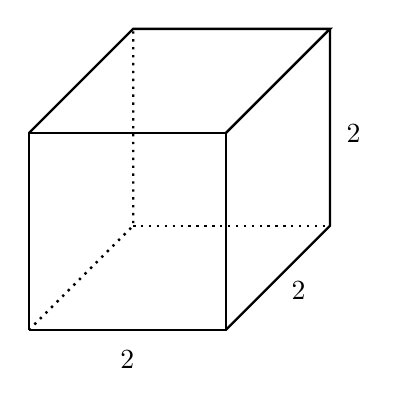
\begin{tikzpicture}[scale=2.5]
	\draw[line width=0.03cm] (0,0) -- (1,0) -- (1,1) -- (0,1) -- (0,0);
	\draw[line width=0.03cm] (0,1) -- (0.53,1.53) -- (1.53,1.53) -- (1,1);
	\draw[line width=0.03cm] (1.53,1.53) -- (1.53,0.53) -- (1,0);
	\draw[line width=0.03cm, dotted] (0,0) -- (0.53,0.53) -- (0.53,1.53);
	\draw[line width=0.03cm, dotted] (0.53,0.53) -- (1.53,0.53);
	\node at (0.5,-0.15) {$2$};
	\node at (1.37,0.2) {$2$};
	\node at (1.65,1) {$2$};
	\end{tikzpicture}
	\] \pspace

\sol The volume of a cube is $s^3$. But then we have\dots
	\[
	V= s^3= 2^3= 8
	\]
The surface area of a cube is $\text{SA}= 6s^2$. But then we have\dots
	\[
	\text{SA}= 6 \cdot 2^2= 6 \cdot 4= 24
	\]
The diagonal of the bottom of the cube is the hypotenuse of the right triangle formed using two sides of the base of the cube. But by the Pythagorean Theorem, we know that $2^2 + 2^2= c^2$. But then $c^2= 4 + 4= 8$ so that $c= \sqrt{8}$. But this hypotenuse is the base of the right triangle with height 2 and hypotenuse the diagonal of the cube. But then by the Pythagorean Theorem, we have $(\sqrt{8})^2 + 2^2= c^2$. But then $c^2= 8 + 4= 12$ so that $c= \sqrt{12}$. 








\end{document}